%\documentclass[10pt,twocolumn,letterpaper,draft]{article}
\documentclass[10pt,letterpaper]{ctexart}

\usepackage{cvpr}
\usepackage{graphicx}
\usepackage{wrapfig}
\usepackage{amsmath}
\newtheorem{myDef}{Definition}
\newtheorem{myTheo}{Theorem}

\usepackage{amssymb}
% \usepackage{color}
\usepackage{subfigure}
\usepackage{algorithm}
\usepackage{algorithmicx}
\usepackage{algpseudocode}
\usepackage{pythonhighlight}
\usepackage{xcolor}
\usepackage{listings}

\lstset{language=C++,
    basicstyle=\ttfamily,
    frame=single,
    keywordstyle=\color{blue}\ttfamily,
    stringstyle=\color{magenta}\ttfamily,
    commentstyle=\color{green}\ttfamily,
    morecomment=[l][\color{magenta}]{\#},
    morekeywords={*,uint_fast64_t}
}

\renewcommand{\labelenumi}{\alph{enumi}.} % Make numbering in the enumerate environment by letter rather than number (e.g. section 6)
\floatname{algorithm}{算法}
\renewcommand{\algorithmicrequire}{\textbf{输入:}}
\renewcommand{\algorithmicensure}{\textbf{输出:}}
\renewcommand{\lstlistingname}{代码清单}

\usepackage{enumitem}
\setenumerate[1]{itemsep=0pt,partopsep=0pt,parsep=\parskip,topsep=5pt}
\setitemize[1]{itemsep=0pt,partopsep=0pt,parsep=\parskip,topsep=5pt}
\setdescription{itemsep=0pt,partopsep=0pt,parsep=\parskip,topsep=5pt}

% Include other packages here, before hyperref.

% If you comment hyperref and then uncomment it, you should delete
% egpaper.aux before re-running latex.  (Or just hit 'q' on the first latex
% run, let it finish, and you should be clear).
\usepackage[pagebackref=true,breaklinks=true,letterpaper=true,colorlinks,bookmarks=false]{hyperref}


\cvprfinalcopy % *** Uncomment this line for the final submission

\def\cvprPaperID{159} % *** Enter the CVPR Paper ID here
\def\httilde{\mbox{\tt\raisebox{-.5ex}{\symbol{126}}}}

\newcommand{\mypara}[1]{\paragraph{#1.}}

\graphicspath{{figures/}}

% Pages are numbered in submission mode, and unnumbered in camera-ready
%\ifcvprfinal\pagestyle{empty}\fi
\setcounter{page}{1}


%\begin{CJK*}{GBK}{song}

\newcommand{\figref}[1]{图\ref{#1}}
\newcommand{\tabref}[1]{表\ref{#1}}
\newcommand{\equref}[1]{式\ref{#1}}
\newcommand{\secref}[1]{第\ref{#1}节}

\ctexset{
  section={
          name={,、},
          number={\chinese{section}},
          format={\heiti},
          beforeskip={0.1ex},
          afterskip={0.1ex},
          aftername={\nobreak},
          indent={\parindent},
          },
}
\usepackage{zhnumber}

\newcommand\zhsubsec[1]{{% 中文小节
\bfseries{
\stepcounter{subsection}(\zhnum{subsection}){#1}}
\vspace{0.1pt}%
}}

%%%%%%%%% TITLE

% \begin{algorithm}
%   \caption{题注}
%     \begin{algorithmic}[1] %每行显示行号
%         \Function {$Function name$}{$parameters$}
%
%         \EndFunction
%     \end{algorithmic}
% \end{algorithm}

\begin{document}
\pagestyle{plain}
\title{
    \begin{center}
        \phantom{Start!}
    	  \vspace{2cm}
        \center{\zihao{1} 中山大学数据科学与计算机学院}
        \center{\zihao{2} 计算机科学与技术专业-人工智能}
        \center{\zihao{2} 本科生实验报告}
        \center{(2018-2019学年秋季学期)}
    \end{center}
}
\maketitle

\begin{center}
    \setlength{\baselineskip}{40pt}
    \vspace{1cm}
    \zihao{-2}
    \center{
        \begin{tabular}{cc}
      	学\qquad 号:& \underline{~~~~~~16337113~~~~~~}  \\
      	姓\qquad 名:& \underline{~~~~~~~劳马东~~~~~~~}  \\
        教学班级:   & \underline{~~~~~教务2班~~~~~}  \\
      	专\qquad 业:& \underline{~~~~~~~~~超算~~~~~~~~}  \\
      	\end{tabular}
    }
\end{center}
\pagebreak

%%%%%%%%% BODY TEXT %%%%%%%%%%%%%%%%%%%%%%%%%%%%%%%%%%%%%%%%
\section{实验题目}
实现6X6的黑白翻转棋的人机对战,要求:
\begin{itemize}[itemindent=1.5em]
  \item 横排、竖排、对角线均可翻转;
  \item 要求使用alpha-beta剪枝;
  \item 搜索深度和评价函数不限,自己设计。在报告中说明清楚自己的评价函数及搜索策略;
  \item 实验结果要求展示至少连续三个回合(人和机器各落子一次指一回合)的棋局分布情况,
  并输出每步落子的得分。
\end{itemize}

\section{实验内容}
\zhsubsec{算法原理}
\begin{enumerate}[itemindent=2.5em,label=\arabic*、]
  \item 博弈树
  \begin{itemize}
      \item 节点:每次落子后棋盘的状态
      \item 行动:在合法的位置落子
      \item 双方轮流扩展节点:两个玩家的的行动逐层交替出现
      \item 评价函数:当前棋盘状态的优劣得分
      \item 节点的值:对游戏双方都最优的子节点的值
  \end{itemize}

    \item $Minimax$搜索
    \par \qquad $Minimax$搜索是一种DFS搜索,在节点的各层,玩家A和玩家B轮流地选择下一层中对自己最有利的
    子节点。不妨假设A选择节点值大的子节点,B选择小的子节点(因为节点值小说明对A不利,换言之对B有利)。
    \par \qquad 如图(a),红色节点表示A的选择,绿色节点表示B的选择。在最底层的叶子节点,节点的值根据评估函数获得,之后,叶子节点的值
    往上传到父节点,绿色节点选择子节点中值最小的作为自己的值,因此绿色节点分别选择了-2和-3,之后,-2和-3传到根节点,选择其中
    最大的一个,即-2作为自己的值。

    \begin{figure}[H]
    \centering
    \subfigure[$Minimax$搜索例子]{
    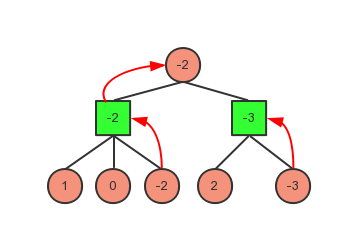
\includegraphics[width=0.4\textwidth]{minimax-example.png}
    \label{fig:minimax-example}}
    \subfigure[$\alpha \beta$剪枝例子1]{
    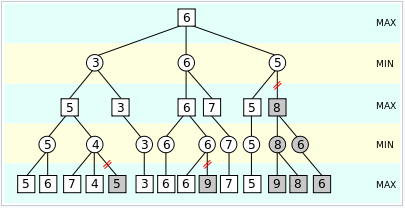
\includegraphics[width=0.5\textwidth]{ab-1.png}
    \label{fig:alphabeta-example1}}
    \end{figure}

    \begin{algorithm}
      \caption{Minimax搜索}
        \begin{algorithmic}[1] %每行显示行号
          \Require $node$当前节点状态,$is\_max$是否极大节点
          \Ensure 博弈树的值
            \Function {minimax}{$node, is\_max$}
              \If {$node$ is a leaf}
                \State \Return {the heuristic value of $node$}
              \Else
                \If {$is\_max$}
                  \State {$value \gets -\infty$}
                  \For {\textbf{each} $child$ of $node$}
                    \State {$value \gets$ max($value$, minimax($child, FALSE$))}
                  \EndFor
                  \State \Return {$value$}
                \Else
                  \State {$value \gets +\infty$}
                  \For {\textbf{each} $child$ of $node$}
                    \State {$value \gets$ min($value$, minimax($child, TRUE$))}
                  \EndFor
                  \State \Return {$value$}
                \EndIf
              \EndIf
            \EndFunction
        \end{algorithmic}
    \end{algorithm}
    
    \newpage
    \item $\alpha \beta$剪枝
    \par \qquad 在博弈树搜索中,有很多节点是没有必要扩展的。例如对于图(b)中的例子,
    DFS搜索到值为5的节点时,就没有必要往下扩展它。因为它的父节点是极小节点,它会选择
    子节点中最小的一个,而前面搜索到的子节点的值4已经传给父节点,5往下扩展必定会使它的值
    >=5,这肯定不会被父节点选择。
    \par \qquad 判断一个节点是否可以剪枝,更普遍的标准是其$\alpha$值大于或等于某个极小祖先节点的$\beta$
    值,或其$\beta$值小于或等于某个极大祖先节点的$\alpha$值。因为对于极小祖先节点A来说,它选择的子节点的值必定比
    它的$\beta$值小,而$\alpha$值大于A的$\beta$的后代节点B就对A的选择没有影响了,极大祖先节点同理。
    $\alpha \beta$剪枝算法的过程是:
    \begin{enumerate}[itemindent=1.5em,label=(\arabic*)]
      \item 每个节点维护两个值——$\alpha$和$\beta$,分别表示
    极大节点已探索的子节点中最大的值和极小节点已探索的子节点中最小的值。
      \item 初始状态下,$\alpha$的值为$-\infty$,$\beta$的值为$+\infty$。
      \item 在扩展子节点的过程中,如果发现$\alpha \geq \beta$,
    就可以停止扩展。因为对于极大节点,继续探索只会使$\alpha$值和节点值更大,而它的父节点会选择一个节点值$\leq \beta$的节点,
    极小节点同理。
    \end{enumerate}
    考虑图(c)-(j)的具体例子,从上至下各层用$r$、$a$、$g$、$p$、$c$标记:
    \begin{enumerate}[itemindent=1.5em,label=(\arabic*)]
      \item 步骤1:初始时所有节点的$\alpha=-\infty$、$\beta=+\infty$;
      \item 步骤2:子节点$c_1$的3传给父节点$p_1$,$p_1$更新$\beta$值为3;
      \item 步骤3:继续探索子节点$c_2$,值为17,比$p_1$的$\beta$值大,不更新$p_1$;
      \item 步骤4:$p_1$节点值确定为3,向上传递给$g_1$,$g_1$更新$\alpha$值为3;
      \item 步骤5:$g_1$带着自己的$\alpha$值向下扩展,探索到$c_3$(值为2),父节点$p_2$更新$\beta$值为2,发现$\alpha \geq \beta$,扩展结束;
      \item 步骤6:$g_1$节点值确定为3,向上传递给$a_1$,$a_1$更新$\beta$值为3,然后带着这个$\beta$值向下探索;
      \item 步骤7:探索节点$c_4$(值为15),更新$p_2$节点值为15,继续往上更新$g_2$的$\alpha$值为15,$g_1$节点值确定为3,$r$确定$\alpha$为3,向下扩展;
      \item 步骤8:$p_4$、$p_5$的过程同理。
    \end{enumerate}

    \begin{figure}[H]
      \centering
      \subfigure[step 1]{
      \includegraphics[width=0.3\textwidth]{1.png}}
      \subfigure[step 2]{
      \includegraphics[width=0.3\textwidth]{2.png}}
      \subfigure[step 3]{
      \includegraphics[width=0.3\textwidth]{3.png}}
      \subfigure[step 4]{
      \includegraphics[width=0.3\textwidth]{4.png}}
      \subfigure[step 5]{
      \includegraphics[width=0.3\textwidth]{5.png}}
      \subfigure[step 6]{
      \includegraphics[width=0.3\textwidth]{6.png}}
      \subfigure[step 7]{
      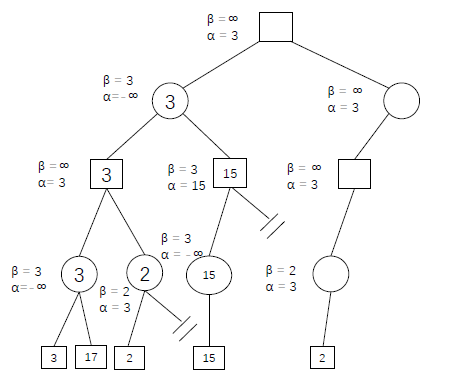
\includegraphics[width=0.3\textwidth]{7.png}}
      \subfigure[step 8]{
      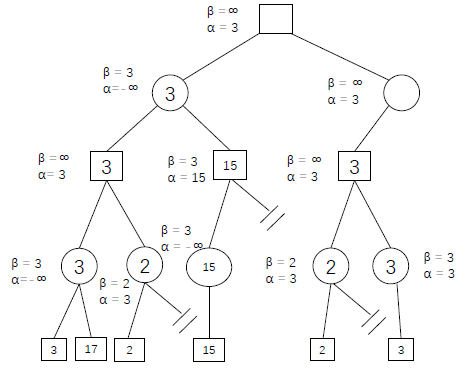
\includegraphics[width=0.3\textwidth]{8.png}}
      \end{figure}

    \begin{algorithm}
      \caption{带$\alpha\beta$剪枝的Minimax搜索}
        \begin{algorithmic}[1] %每行显示行号
          \Require $node$当前节点状态,$alpha$节点的$\alpha$值,$beta$节点的$\beta$值,$is\_max$是否极大节点
          \Ensure 博弈树的值
            \Function {minimax\_with\_alphabeta}{$node, alpha, beta, is\_max$}
              \If {$node$ is a leaf}
                \State \Return {the heuristic value of $node$}
              \Else
                \State ...
                \For {\textbf{each} $child$ of $node$}
                  \State $score \gets$ minimax\_with\_alphabeta($child, alpha, beta, FALSE$)
                  \If {$is\_max$}  
                    \State {$value \gets$ max($value, score$)}
                    \State $alpha \gets$ max($alpha, value$)
                  \Else
                    \State {$value \gets$ min($value, score$)}
                    \State $beta \gets$ min($beta, value$)
                  \EndIf
                  \If {$alpha \geq beta$}
                    \State \textbf{break}
                  \EndIf
                \EndFor
                \State \Return {$value$}
              \EndIf
            \EndFunction
        \end{algorithmic}
    \end{algorithm}

    \item $Negamax$搜索
    \par \qquad $Minimax$算法的代码太过冗余,$Negamax$对其进行简化。该算法基于max($a,b$) == -min($-a, -b$)的事实来简化代码实现,
    即玩家A的节点值相当于玩家B节点值的负数。
    \begin{algorithm}
      \caption{$Negamax$搜索}
        \begin{algorithmic}[1] %每行显示行号
          \Require $node$当前节点状态,$factor$极大节点取值1,极小取值-1
          \Ensure 博弈树的值
            \Function {negamax}{$node, factor$}
            \If {$node$ is a leaf}
              \State \Return {$factor \times$ the heuristic value of node}
            \Else
              \State {$value \gets -\infty$}
              \For {\textbf{each} $child$ of $node$}
                \State {$value \gets$ max($value$, -negamax($child, -color$))}
              \EndFor
              \State \Return {$value$}
            \EndIf
            \EndFunction
        \end{algorithmic}
    \end{algorithm}

    \item 带$\alpha \beta$剪枝的$Negamax$搜索
    % \par \qquad 为什么递归中传递的是$-\beta_p$作为子节点的$\alpha_c$,$-\alpha_p$作为子节点的$\beta_c$?
    % 假设当前节点时极大节点,那么它的子节点是极小节点,子节点在循环中更新它的$\beta_c$值,
    % 即$\beta_c=$ min($\beta_c, value$),等价于$\beta_c=$ -max($-\beta_c, -value$)
    \begin{algorithm}
      \caption{带$\alpha \beta$剪枝的$Negamax$搜索}
        \begin{algorithmic}[1] %每行显示行号
          \Require $node$当前节点状态,$alpha$节点的$\alpha$值,$beta$节点的$\beta$值,$factor$极大节点取值1,极小取值-1
          \Ensure 博弈树的值
            \Function {negamax\_with\_alphabeta}{$node, alpha, beta, factor$}
              \State {...}
              \For {\textbf{each} $child$ of $node$}
                \State {$value \gets$ max($value$, -negamax\_with\_alphabeta($child, -beta, -alpha, -color$))}
                \State $alpha \gets$ max($alpha, value$)
                \If {$alpha \geq beta$}
                  \State \textbf{break}
                \EndIf
              \EndFor
              \State \Return {$value$}
            \EndFunction
        \end{algorithmic}
    \end{algorithm}
    % \item 探索深度的控制
    % \par \qquad 如果一直探索到游戏结束的状态,博弈树搜索总能找到对自己最优的落子位置。
    % 但是,每向下扩展一层,需要探索的节点数就呈指数级别增长($b^d$),这是很可怕的,相当耗时,
    % 因此需要限制搜索的深度。
    % \par \qquad 最简单的做法是固定一个最大深度,但是事实告诉我,棋盘上落子越多,算法搜索的速度
    % 越快,因为节点的平均分支数$b$减少了。因此,每一层可以设置一个固定的往下探索的总节点数$k_i$,
    % 对于该层一个具有$b_j$个分支的节点,探索深度就是$d_j = \min\{d_{parent} - 1, \log_{b_j}k_i(b_j > 0)\}$。
    % \begin{figure}[H]
    %   \centering
    %   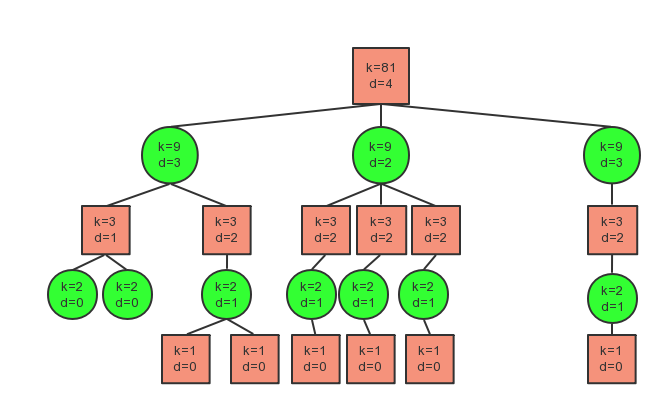
\includegraphics[width=0.8\textwidth]{depth.PNG}
    %   \caption{深度控制示例}
    % \end{figure}
    \item 动态规划
    \par \qquad {\color{red}在搜索过程中,有很多子问题重复出现,因此可以用一个表格记录已搜索节点的节点值,下一次遇到时直接查表
    而无需搜索}。实验中发现,不使用动态规划前,6X6棋盘每次落子搜索时间很长(等了十几分钟还没得到解),而加上动态规划之后
    能在十几秒以内得到解。
    \item 评估函数的设计
      \begin{enumerate}[itemindent=2.5em,label=(\arabic*)]
        \item 棋子数之差
        \par \qquad 计算棋盘上先手棋子数与后手棋子数之差。
        \item sigmoid函数
        \par \qquad sigmoid函数的作用是将取值为$(-\infty, +\infty)$的数映射到$(0, 1)$。
        评估函数首先统计棋盘上先手棋子和后手棋子个数,然后计算各自的sigmoid值,作为棋盘得分。
      \end{enumerate}
\end{enumerate}

\section{关键代码}
\begin{enumerate}[itemindent=2.5em,label=\arabic*、]
  \item Minimax搜索
  \par \qquad 代码中,初始化部分获取当前节点的棋子(对于极大节点是先手棋子,极小节点是后手棋子)。
  之后,获取在当前状态下能够落子的位置,而不是生成当前节点的后继状态,避免拷贝。如果无法落子,说明游戏结束,
  就返回对当前棋盘的评分,否则递归地扩展每一种落子位置。
  \par \qquad 递归完成之后回溯,恢复被翻转的棋子,尝试下一种落子。
  更新这些落子选择中最优的方案和$\alpha$、$\beta$值,在$\alpha \geq \beta$时停止扩展。除最优得分外,函数
  还需要记录最优落子位置,因为最顶层函数调用的目的就是要知道怎么落子。
  \newpage
  \begin{python}
def minimax(self, remain_depth, alpha, beta, is_max):
  ... # 一些初始化,获得极大极小节点的棋子
  moves_list = self._board.generate_moves(char)   # 当前可落子的位置
  if remain_depth == 0 or not moves_list:   # 到达设定深度或无法落子
      best_score = self._evaluation(self._board)
  else:
    for move in moves_list:
      all_reverse = self._board.apply_move(move, char, False)   # 落子,返回被翻的棋子
      score = self.minimax(remain_depth - 1, alpha, beta, not is_max)[0]
      for p in all_reverse:   # 回溯
          self._board[p] = opp_char
      if all_reverse:
          self._board[move] = Board.BLANK
      if is_max:    # alpha节点,选择较大的值
          if chosen_score > best_score:
              best_score = chosen_score
              best_move = move
          alpha = max(alpha, best_score)
      else:         # beta节点,选择较大的值
          if chosen_score < best_score:
              best_score = chosen_score
              best_move = move
          beta = min(beta, best_score)
      if alpha >= beta:   # alpha >= beta停止扩展
          break
    return best_score, best_move
\end{python}
  
  \item Negamax搜索
  \par \qquad Negamax搜索的代码比Minimax搜索简洁,它不需要判断当前节点时极大节点还是极小节点,因为
  二者本身可以通过max($a,b$) = $-$min($-a, -b$)这一公式转换。$color$变量取值$\pm 1$,极大节点为1,
  极小节点为-1,因为极小节点处的棋盘得分需要乘上-1才能转化为极大节点得分。值得注意的是,父节点的
  $-\beta$、$-\alpha$值传递给子节点作为$\alpha$和$\beta$值。
\begin{python}
def negamax(self, remain_depth, alpha, beta, color):
  ...
  best_score = -self.INF
  moves_list = self._board.generate_moves(char)
  if remain_depth == 0 or not moves_list:
      best_score = color * self._evaluation(self._board)
  else:
    for move in moves_list:
      all_reverse = self._board.apply_move(move, char, False)
      chosen_score = self.negamax(remain_depth - 1, -beta, -alpha, -color)[0]
      ... # 回溯
      if best_score < -chosen_score:
          best_score, best_move = -chosen_score, move
      alpha = max(alpha, best_score)
      if alpha >= beta:
          break
  return best_score, best_move
\end{python}
  \item 动态规划
  \begin{enumerate}[itemindent=3.5em,label=(\arabic*)]
    \item 搜索前
      \begin{python}
  s_board = str(self._board)
  entry = self._table.get(s_board, None)
  if entry is not None and entry.depth >= remain_depth:
      if entry.flag == Flag.VALUE:    # 保存的是节点值,返回节点值和落子
          return entry.value, entry.move
      elif entry.flag == Flag.ALPHA:   # 保存的是alpha或beta,更新alpha、beta
          alpha = max(alpha, entry.value)
      else:
          beta = min(beta, entry.value)
      if alpha >= beta:
          return entry.value, entry.move
  alpha_orig = alpha
  beta_orig = beta
      \end{python}
    \item 搜索后
      \begin{python}
  entry = Entry()
  # 最终的best_score一定等于最终的alpha值或beta值
  entry.value = best_score
  entry.move = best_move
  entry.depth = remain_depth
  if entry.value <= alpha_orig:
      entry.flag = Flag.BETA
  elif entry.value >= beta_orig:
      entry.flag = Flag.ALPHA
  else:
      entry.flag = Flag.VALUE
  self._table[s_board] = entry
      \end{python}
  \end{enumerate}
\end{enumerate}

\section{创新点\&优化}
\begin{enumerate}[itemindent=2.5em,label=\arabic*、]
  \item 实现了带$\alpha \beta$剪枝的Negamax算法;
  \item 使用动态规划,以空间换时间,使算法可短时间内搜索到游戏结束,保证选择最优子节点。
\end{enumerate}

\section{实验结果及分析}
下列图中,O表示先手,X表示后手,+表示提示可以落子的位置,得分是O棋子与X棋子之差。
图(k)表示当前O有4处落子位置。下面展示开始的三个回合,更详细完整的对战过程在result文件夹下。
\begin{figure}[H]
  \centering
  \subfigure[初始状态]{
  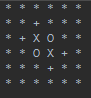
\includegraphics[width=0.15\textwidth]{play/0.png}}
\end{figure}

\begin{enumerate}[itemindent=2.5em,label=\arabic*、]
  \item 第一回合:玩家1下在(1,2)位置,翻一个X,得分3;玩家2下在(3,1)位置,翻一个O,得分0;
  \item 第二回合:玩家1下在(4,3)位置,翻一个X,得分3;玩家2下在(0,2)位置,翻两个X,得分-2;
  \item 第三回合:玩家1下在(0,1)位置,翻一个X,得分1;玩家2下在(0,0)位置,翻一个O,得分-2;
\end{enumerate}


\begin{figure}[H]
  \centering
  \subfigure[round 1-player1]{
  \includegraphics[width=0.2\textwidth]{play/1.png}}
  \subfigure[round 1-player2]{
  \includegraphics[width=0.2\textwidth]{play/2.png}}
  \subfigure[round 2-player1]{
  \includegraphics[width=0.2\textwidth]{play/3.png}}
  \subfigure[round 2-player2]{
  \includegraphics[width=0.2\textwidth]{play/4.png}}
  \subfigure[round 3-player1]{
  \includegraphics[width=0.2\textwidth]{play/5.png}}
  \subfigure[round 3-player2]{
  \includegraphics[width=0.2\textwidth]{play/6.png}}
\end{figure}
\end{document}
